\newpage
\section{Model analityczny}

Celem stworzonego w niniejszym rozdziale modelu analitycznego jest
zdefiniowanie, jak wyglądać będzie architektura tworzonego systemu, jakie
problemy mogą być związane z poszczególnymi elementami całości i jakie kroki
można przedsięwziąć w celu zapobieżenia najczęściej występującym i najbardziej
prawdopodobnym zagrożeniom. Aby to osiągnąć, zaprezentowano różnego rodzaju
diagramy UML, które służą jako wizualna reprezentacja architektury systemu i
pozwalają na łatwiejszą analizę stanu projektu.


Przedstawiony na poniższym obrazku diagram klas reprezentuje wszystkie
wykorzystywane przez Zleceniodawcę elementy składające się na cały system.
Diagram ten ma znaczenie przede wszystkim dla deweloperów i osób zajmujących się
wytwarzaniem oprogramowania, tym niemniej powinien zostać zatwierdzony przed
przedstawicieli Zleceniodawcy - diagram klas jest bowiem punktem łączącym z
jednej strony wyobrażenie klienta o podziale funkcjonalności a z drugiej decyzje
projektowe podjęte przez zespół zajmujący się implementacją.

Diagram klas powinien obrazować zależności (agregacje, kompozycje, relację
dziedziczenia) pomiędzy poszczególnymi klasami na tyle szczegółowo, by osoby 
nieposiadające wykształcenia informatycznego i nieznające metod programowania
obiektowego mogłby zrozumieć zasadę podziału bez szczegółowych wyjaśnień. Z
tego też powodu na poniższym rysunku skoncentrowano się na powiązaniach pomiędzy
poszczególnymi klasami a nie na nazywaniu i przedstawianiu atrybutów i metod
poszczególnych klas. Nie stanowią one żadnej wartości z punktu widzenia
Zleceniodawcy a mogą stanowić ograniczenie i usztywnienie schematu dla
deweloperów, którzy lepiej znają metody dostarczania funkcjonalności i będą
mogli lepiej modyfikować schemat w zależności od potrzeb, nie naruszając
jednocześnie warunków umowy. Wszystkie atrybuty czy operacje ważne z punktu
widzenia Zleceniodawcy, które mogą mieć wpływ na ocenę projektu zostały
umieszczone na diagramie.

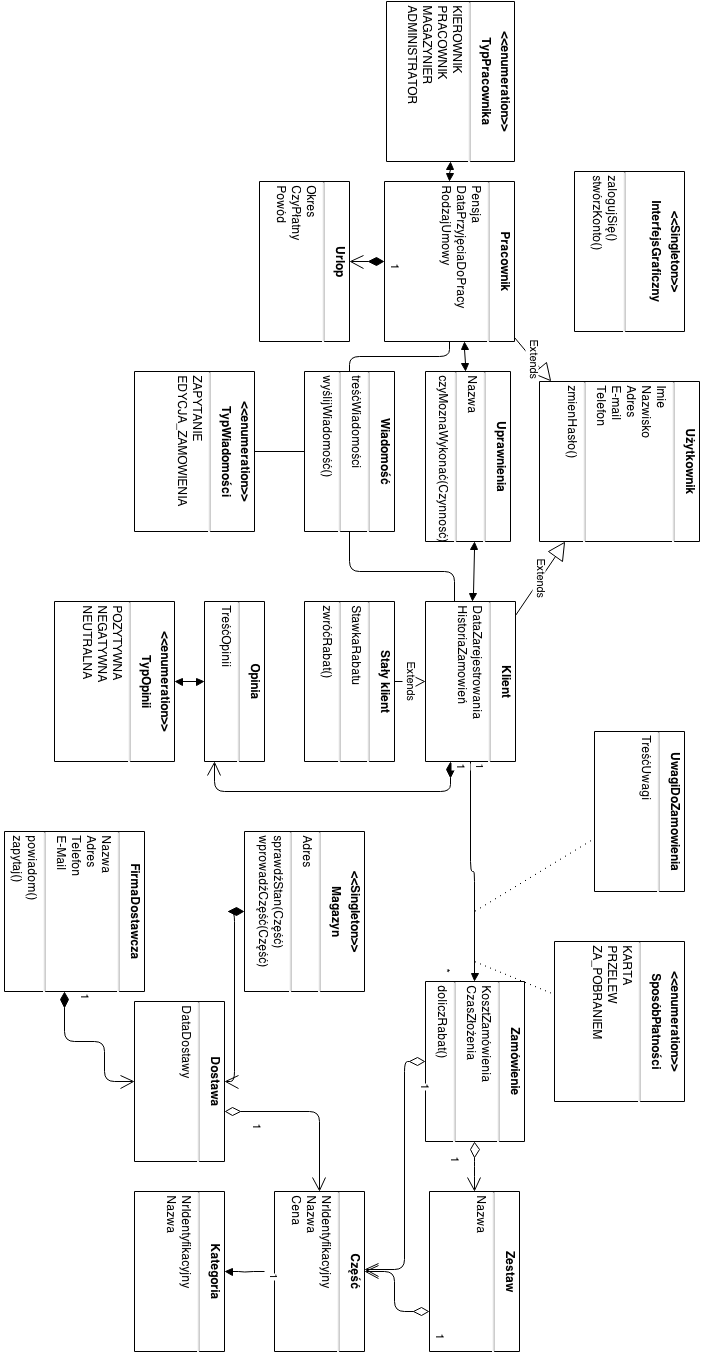
\includegraphics[width=\textwidth,
height=0.8\textheight]{graphics/ClassDiagram.png}


\newpage
Opis klas na przedstawionym diagramie:

\begin{description}
	\item[Użytkownik] \hfill \\
		Klasa abstrakcyjna, będąca bazową dla klas Klient i Pracownik, przechowuje
		informacje dotyczące danej osoby - imię, nazwisko, adres e-mail itp.
	\item[Pracownik] \hfill \\
	 	Osoba z obsługi sklepu, odpowiedzialna za realizację i zarządzanie
	 	zamówieniami
	\item[Stały klient] \hfill \\
		Osoba charakteryzująca się dużą liczbą zamówień bądź długim czasem obecności
		na stronie (czas liczony od czasu rejestracji)
	\item[Klient] \hfill \\
		Osoba składająca zamówienia w sklepie, edytująca swoje zamówienia i opłacająca
		je
	\item[Typ pracownika] \hfill \\
		Enumeracja, będąca oznaczeniem rodzaju pracownika (Szeregowy Pracownik,
		Kierownik itp.)
	\item[Urlop] \hfill \\
		Obsługa urlopów dla pracowników pod kątem czasu ich trwania, momentu ich
		rozpoczęcia (i zakończenia) itp.
	\item[Uprawnienia] \hfill \\
		Obsługa uprawnień zarówno dla pracowników jak i klientów. Pozwala na
		ustalanie, kto ma jakie uprawnienia do edycji i podglądu danych
	\item[Wiadomość] \hfill \\
		Treści przesyłane pomiędzy pracownikami i klientami, służące do przekazywania
		informacji na temat zamówień
	\item[Typ wiadomości] \hfill \\
		Enumeracja, jaki rodzaj wiadomości jest przekazywany (Zapytanie, Edycja
		Zamówienia itp.)
	\item[Opinia] \hfill \\
		Tekst na temat zamówienia, ocena poprawności i jakości realizacji zamówienia
	\item[Typ opinii] \hfill \\
		Enumeracja, jaka opinia została wydana (Pozytywna, Negatywna, Neutralna)
	\item[Zamówienie] \hfill \\
		Informacje na temat złożonego przez klienta Zamówienia
	\item[Uwagi do zamówienia] \hfill \\
		Wszelkiego rodzaju informacje, jakie klient chce zawrzeć w momencie złożenia
		zamówienia - na przykład zaznaczanie wysyłki jako prezent, ustalenie, przed
		jakim terminem zamówienie nie powinno być wysłane, czy możliwy jest odbiór
		osobisty itp.
	\item[Sposób płatności] \hfill \\
		Informacja, jak użytkownik chce zapłacić za złożone zamówienie - inaczej
		wygląda procesowanie zapłaty kartą (wysłanie następuje dopiero po wpłynięciu
		pieniędzy, opłata za pobraniem jest uiszczana dopiero po wysłaniu)
	\item[Część] \hfill \\
		Pojedyncza część rowerowa wraz z informacjami na jej temat - rozmiar, nazwa,
		cena itp.
	\item[Zestaw] \hfill \\
		Złożenie kilku części w jeden, funkcjonalnie sprawny rower. Przechowuje
		informację o tym, jakie części są wymagane, ile ma ich być (rama - 1, pedały
		-2, przerzutki - nieokreślone)
	\item[Kategoria] \hfill \\
		Informacja, do jakiej kategorii zaliczana jest dana część. Jest to pomocne do
		układania zestawów i sprawdzania ich poprawności
	\item[Dostawa] \hfill \\
		Informacje na temat jednej dostawy, jakie części i w jakiej ilości zostały
		dostarczone i kiedy
	\item[Firma dostawcza] \hfill \\
		Informacje na temat firmy, która dostarcza części - dane kontaktowe, adres
		oraz jakie części są w stanie dostarczyć
	\item[Magazyn] \hfill \\
		Klasa pozwalająca na zarządzanie częściami przechowywanymi w magazynie,
		sprawdzanie ich dostępności oraz aktualizacja stanu
	\item[Interfejs graficzny] \hfill \\
		Klasa będąca ``wejściem'' do diagramu klas, odpowiedzialna za podstawową,
		wstępną integrację z użytkownikiem
\end{description}